\scanpage{65}
% upper synoptic diagram; read branches from the common middle object
\diagram{\begin{tikzcd}[ampersand replacement=\&,row sep=small,column sep=small]
\parbox{5.4cm}{polygones pythagoriciens\\ \deleted{\unsure{on}}}\arrow[d,leftright] \& \\
\parbox{5.4cm}{\deleted{\uline{certains}} $(\underline{\lambda_0},\underline{\lambda_1},\beta=\underline{\zeta}(\lambda_0-1)(\lambda_1-1)$}
\arrow[d,leftright] \& \\
\parbox{5.4cm}{\uline{\unsure{certains}} couples de 2 ps. réfl. $\tau_0,\tau_1$ dans \inserted{plan} vectoriel $V$ (épinglé par deux vecteurs $a_0\in V^{\tau_0}\ldots$) : conditions de non dég. et d'engendrer d'un groupe fini \ldots}
\arrow[r,leftright] \&
\left\{\parbox{4.6cm}{\deleted{certains \unsure{couples|pythag.}} \inserted{couples} pythagoriciens $(\tau_0^{C},\tau_1^C)$ dans plan proj. $+\,a_0$ point fixe de $\tau_0^C$, $a_1$ pt fixe de $\tau_1^C$}\right.
\arrow[d,leftright]\\
\&\parbox{4.6cm}{\(\left.\begin{array}{c}\text{Ceci décrit}\\\text{la situation}\\\text{pyth. }\text{\uline{projective}}\end{array}\right\}\) donnée des $K_0,K_1,K$ adm.\\ $+\,a_0,a_1$ ds le syst. défini par $K_0,K_1,K$}
\end{tikzcd}}

% small incidence sketch under the left branch
\diagram{\begin{tikzcd}[ampersand replacement=\&,column sep=small,row sep=small]
V\&L_0\arrow[d,dash]\arrow[dr,dash]\&L_1\arrow[d,dash]\\
\&L'_0\&L'_1
\end{tikzcd}}

% middle left
Si $K_i$ fixé, $\lambda_i$ s'en déduit comme \uline{une} des deux solutions de
\[
\lambda_i^2\unsure{-|+}K_i\lambda_i+1=0
\]
le choix des $\deleted{\unsure{K_i}}\lambda_i$ \uline{équivaut}, \deleted{au choix} \inserted{pour} $\lambda_i\ne-1$ i.e. $K_i\ne-2$ i.e. $\nu_i\ne2$, au choix des $a_i$. \deleted{\unsure{en dehors}} Si par contre $\nu_i=2$ i.e. $\lambda_i=-1$ i.e. $K_{\unsure{i|1}}=\unsure{2|-2}$,
\begin{center}\rule{.8\linewidth}{.3pt}\end{center}

% lower working, written upside down; in its own reading order
\[
\left\{\begin{aligned}
\rho(\unsure{\cdot}e_0)&=\deleted{\unsure{e_1|e_0}}\quad\unsure{\varphi|\rho}(e_1)=-e_1\\
\rho'(\unsure{c|e}_0)&=\unsure{\cdot}
\end{aligned}\right.
\]
\[
\begin{aligned}
(\varepsilon_1,\varepsilon_2)^{\deleted{\unsure{2}}}&=g&
g^{\unsure{2|\prime}}&=\mathrm{id}&g'{}^2&=\mathrm{id}&g''{}^2&=\mathrm{id}\\
(\deleted{\unsure{\varepsilon}}\varepsilon'_1,\varepsilon'_2)&=g'&
gg'&=?&g'g''&=?\\
(\varepsilon_3,\varepsilon'_3)&=g''&gg'g''&=
\end{aligned}
\]
\figure{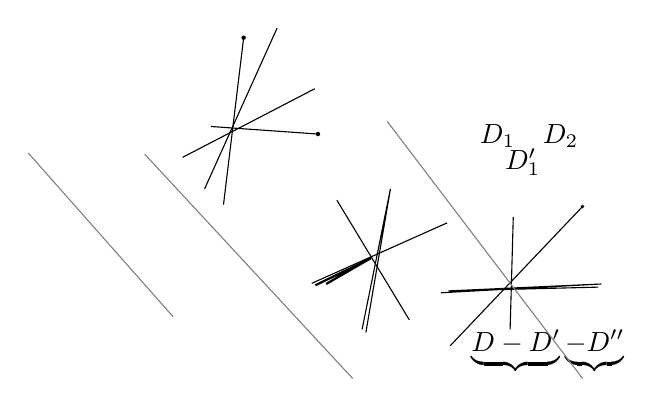
\begin{tikzpicture}[x=.8cm,y=.8cm]
\begin{scope}[shift={(0,2.0)}]
\draw (-.2,-1.2)--(.12,1.45); \fill (.12,1.45) circle (.035);
\draw (-.5,-.95)--(.65,1.6); \draw (-.85,-.45)--(1.25,.64);
\draw (-.4,.04)--(1.3,-.08); \fill (1.3,-.08) circle (.035);
\end{scope}
\begin{scope}[shift={(2.2,-.05)}]
\draw (-.2,-1.13)--(.25,1.1)--(-.14,-1.18);
\draw (-.6,.92)--(.55,-.98); \draw (-1.0,-.40)--(1.15,.56);
\draw[thick] (-.94,-.43)--(-.06,0)--(-.77,-.41);
\end{scope}
\begin{scope}[shift={(4.35,-.55)}]
\draw (-1.1,-.05)--(1.45,.09)--(-.98,-.02)--(1.4,.04);
\draw (0,-.63)--(.05,1.15); \draw (-.95,-.89)--(1.15,1.32);
\fill (1.15,1.32) circle (.03);
\node[above] at (.3,2.1){$D_1\quad D_2$};
\node[above] at (.2,1.65){$D'_1$};
\node[below] at (.6,-.48){$\underbrace{D-D'}\underbrace{-D''}$};
\end{scope}
\draw[thin,gray] (-3.3,1.62)--(-1.0,-.98);
\draw[thin,gray] (-1.45,1.60)--(1.85,-1.96);
\draw[thin,gray] (2.4,2.12)--(5.5,-1.96);
\end{tikzpicture}}
\[
\begin{aligned}
\lambda_0&=\varphi_0^2=(s_0+ic_0)^2=\deleted{\unsure{2}}\underbrace{s_0^2-c_0^2}_{\deleted{\unsure{C}}C_0}+2is_0c_0\\
&&&\hspace{4.5cm}{}+iS_0\\
\lambda_1&=\varphi_1^2=\\
\lambda_0&
\end{aligned}
\]
% archive sheet number: 64
